\section*{Analysis}
\label{sec:analysis}

We run the benchmarks on 4 different hardware.
Two of the devices (Nexus5 and GalaxyNexus) are phones, while the other two are tablets.
The hardware specification is shown in Table~\ref{table:hardware}.
The devices also have different software capabilities: the Nexus 7
  is the only one capable of running OpenCL currently --- since it is the only
  one that's hacked to do so.

\begin{table}[h]\small
\centering
\begin{tabular}{ | l | p{2.5cm} | p{1.75cm} | c |}
    \hline 
    Name & CPU & GPU & Memory \\ \hline
    GalaxyNexus & ARMv7, 2 cores, 1200 Mhz, SIMD NEON & PowerVR-SGX 540 & 694Mb \\ \hline
    Nexus5 & Qualcomm Snapdragon S4 Pro 1.5GHz & Adreno 320 400MHz & 2Gb \\ \hline
    Nexus7 & Qualcomm Snapdragon 800 2.26GHz & Adreno 330 450MHz & 2Gb \\ \hline
    SM-T900 & QuadCore 1.9GHz Cortex-A15 & Mali T628 MP6 & 3Gb \\ \hline
    \hline
\end{tabular}
\caption{The hardware specifications of the devices we ran the benchmarks on. Two of the devices (Nexus 7 and GalaxyNexus) are mobile phones while the other two are tablets.}
\label{table:hardware}
\end{table}

Figure~\ref{fig:benchmarks} shows the output of the benchmarks run~\footnote{We would like to know how we can present these results better}.
Each benchmark is run across the implementd implementations (Java, ThreadedJava, RenderScript, and OpenCL) as well as (when available) across runtimes provided by Android (ART and Dalvik).
All runtimes are normalized to the Java(Dalvik) runtime.

We omit the IO time, since it skews the graph --- in general IO takes 
  order of magnitude more time than the compute part.
We expect the allocate time to be equal across benchmarks, since
  that code is shared across implementations.
Each compute part of the implementation is run 5 times, and we 
  take the minimum value across the runs.
In some cases timer information is not available, for example the compute times for some of the Stencil implementations, this is due to a bug in our code (we omitted inserting the compute timer code) and has been fixed, but we were not able to rerun the benchmarks (primarily due to the IO runtime).

The ART, introduced but disabled in 4.4.2, runtime performs ahead of
  time JIT-ing, while Dalvik uses a traditional hotspot runtime JIT architecture.
It is not clear if ART gives a performance increase, there is massive degradation
  in speed for the Stencil and CUTCP benchmark, for example, which, time permitting, we could
  analyze.

\begin{figure}%
    \centering
    \subfigure[VectorAdd]{{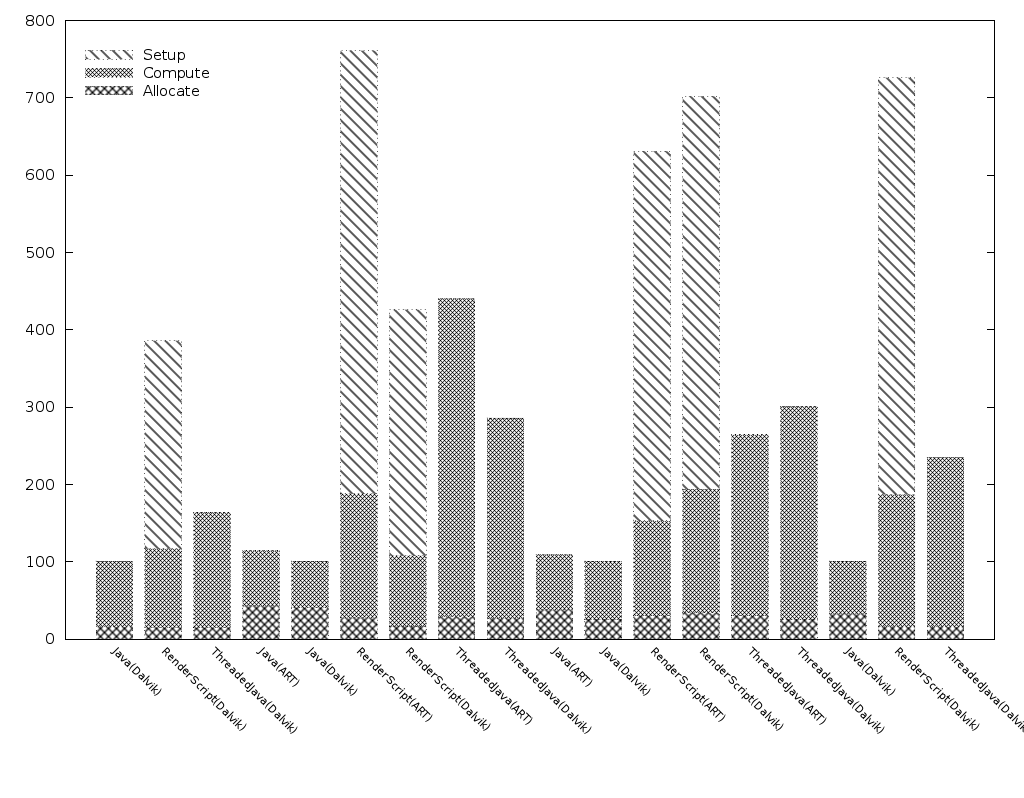
\includegraphics[width=0.5\linewidth]{vecadd} }}~
    \subfigure[SGEMM]{{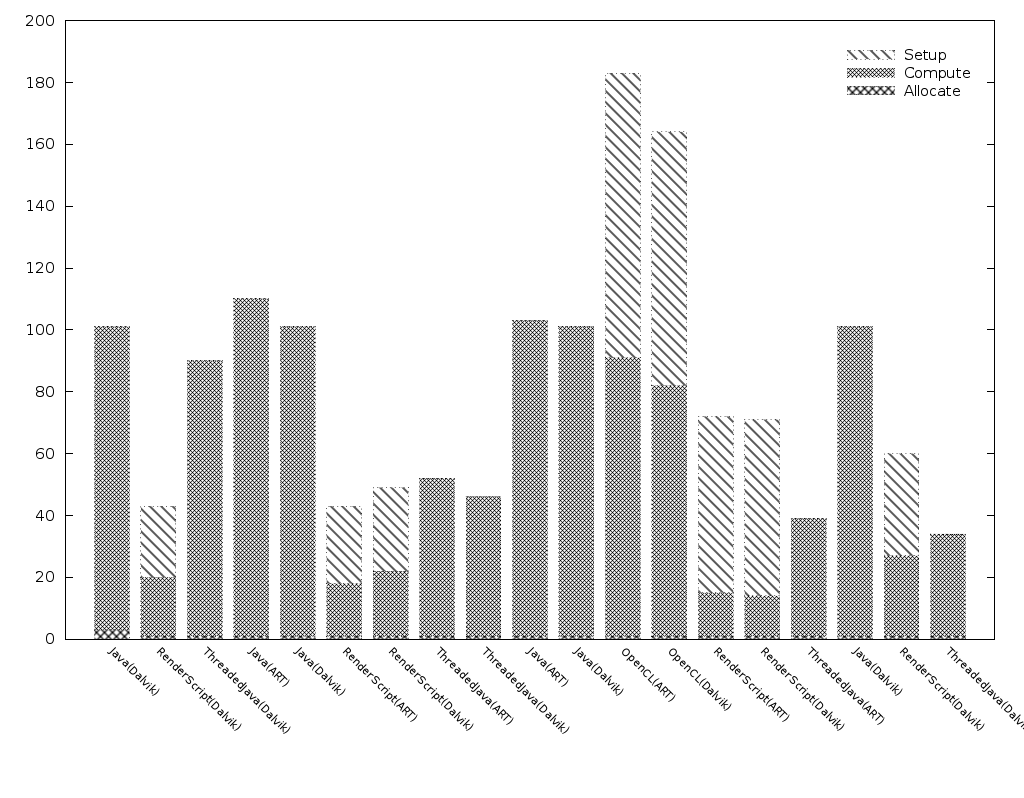
\includegraphics[width=0.5\linewidth]{sgemm} }}\\
    \subfigure[MRI-Q]{{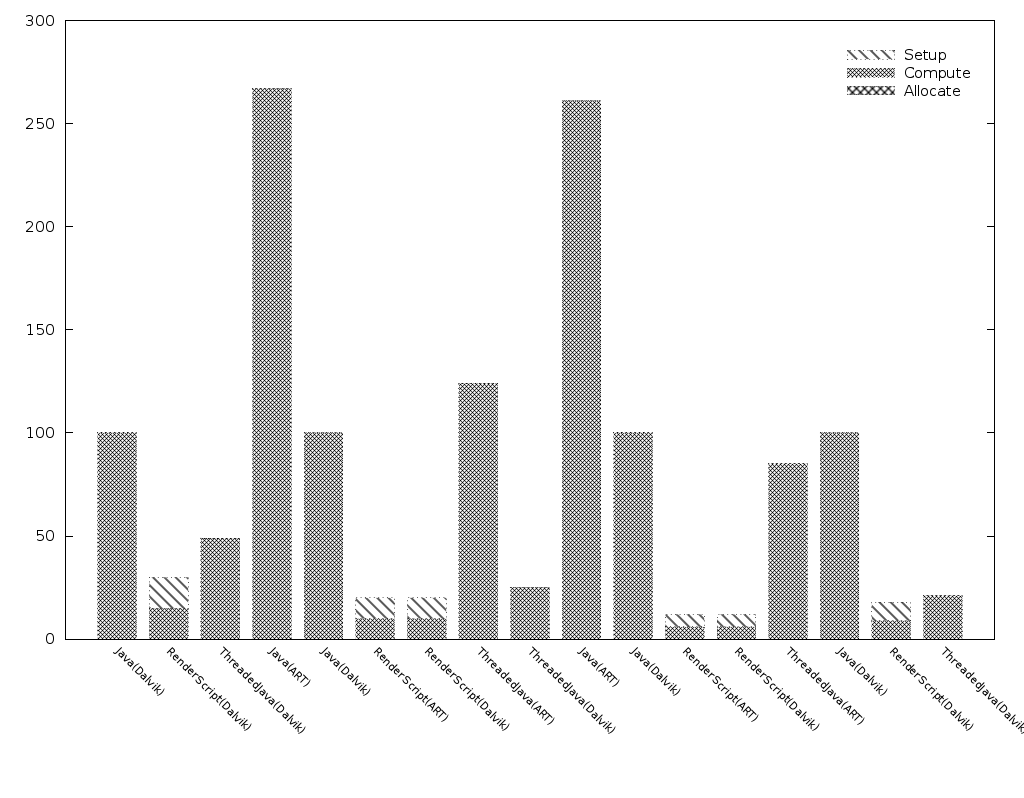
\includegraphics[width=0.5\linewidth]{mriq} }}~
    \subfigure[TPACF]{{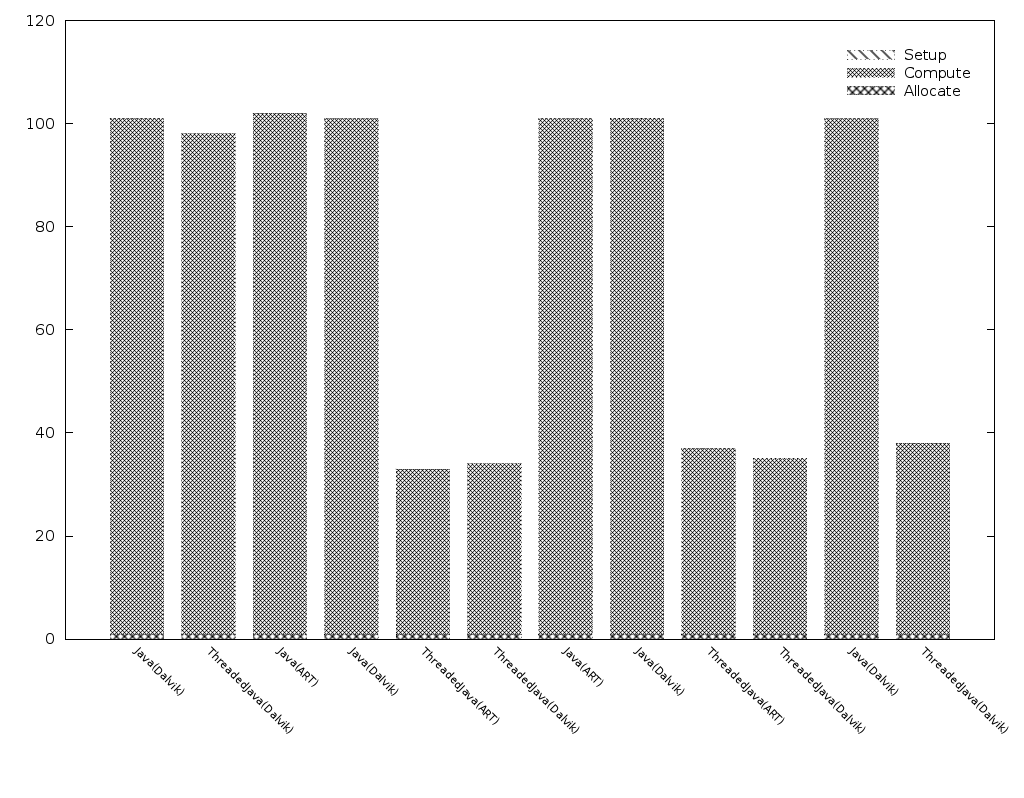
\includegraphics[width=0.5\linewidth]{tpacf} }}\\
    \subfigure[Stencil]{{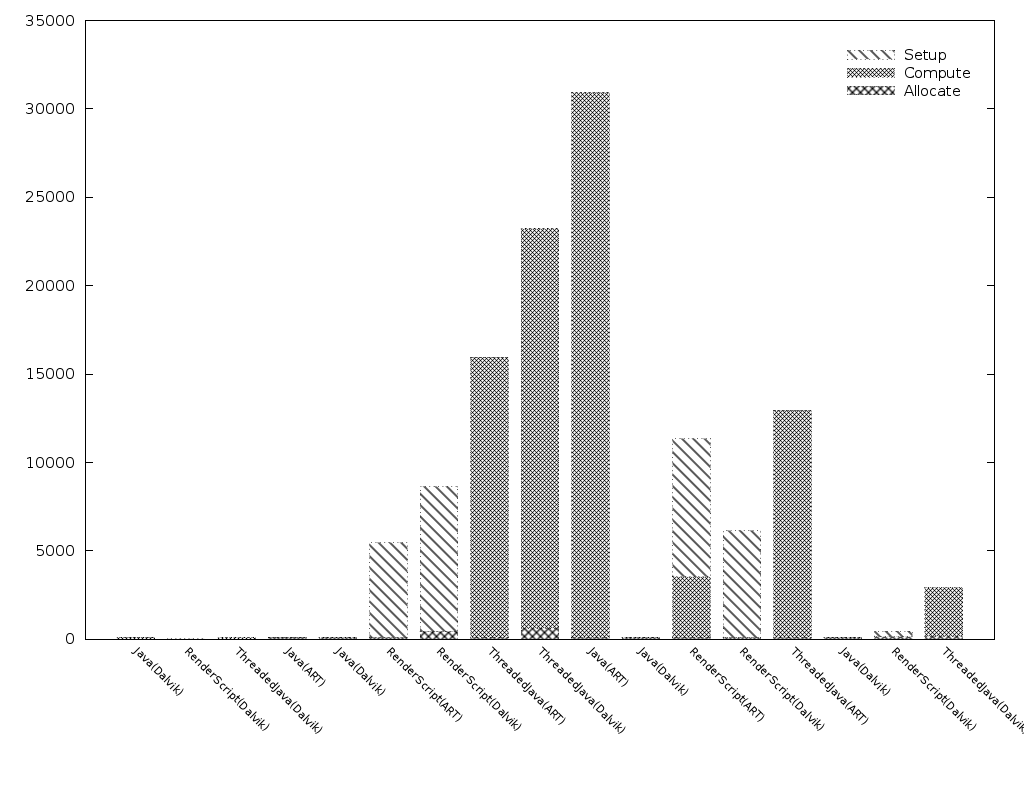
\includegraphics[width=0.5\linewidth]{stencil} }}~
    \subfigure[Histogram]{{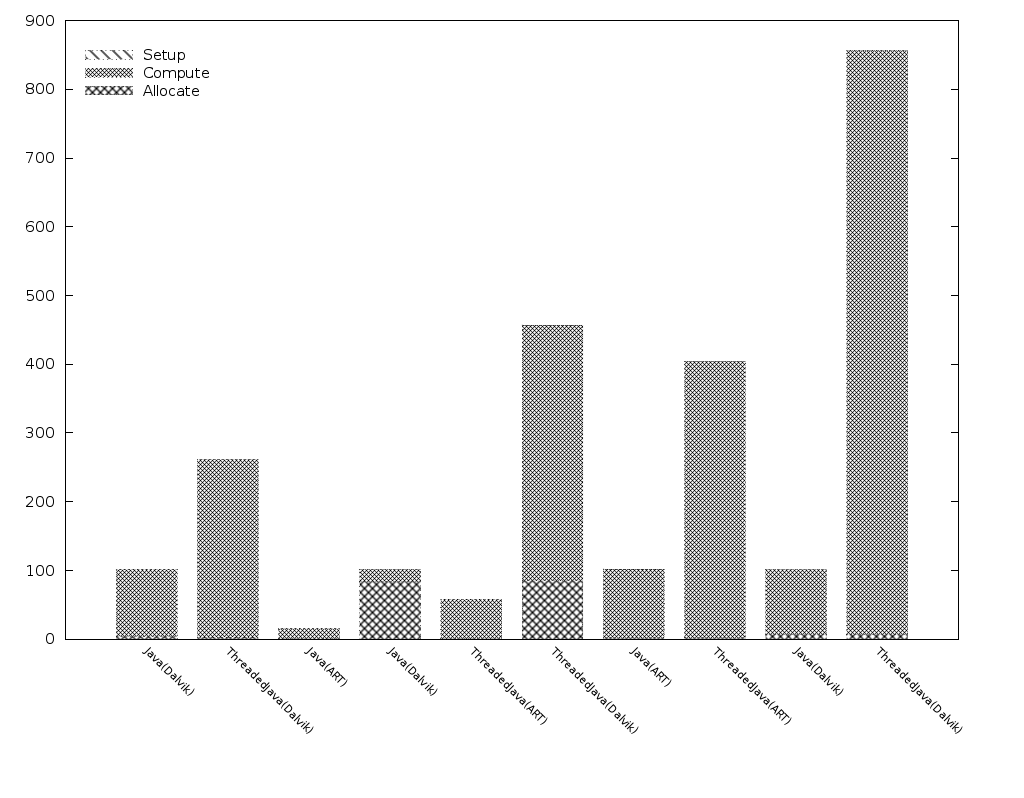
\includegraphics[width=0.5\linewidth]{histogram} }}\\
    \subfigure[CUTCP]{{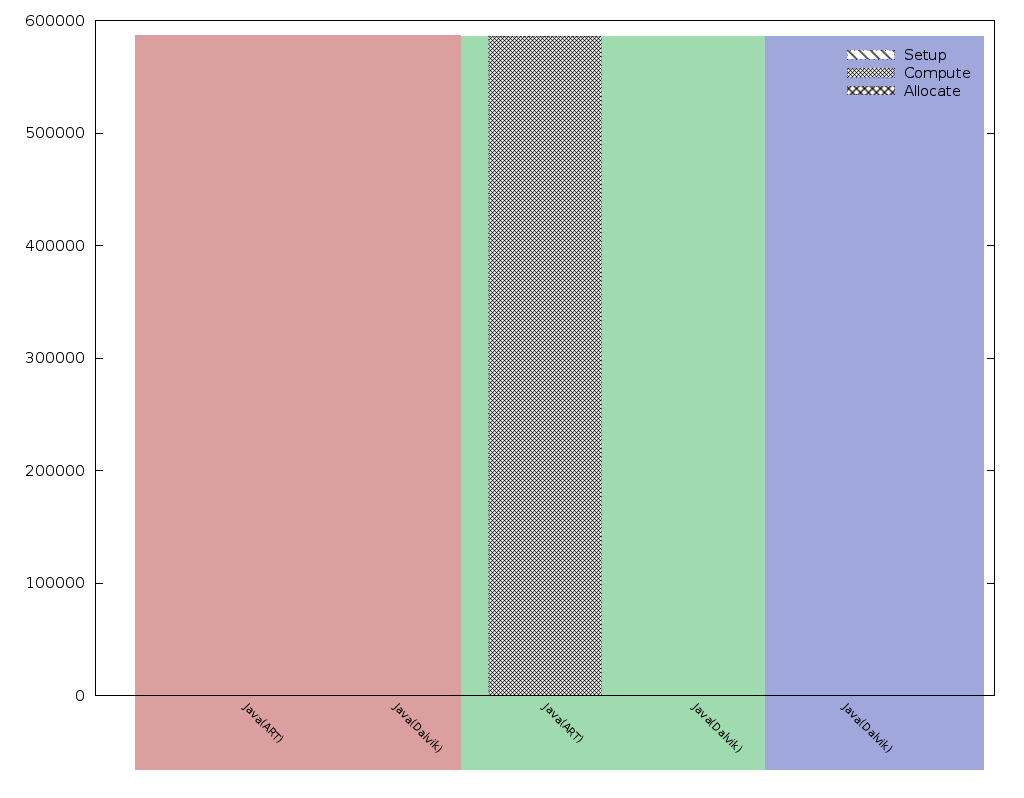
\includegraphics[width=0.5\linewidth]{cutcp} }}%
    \caption{Benchmark results: yellow corresponds to runs being performed on GalaxyNexus, Red on the Nexus 5, Green on the Nexus 7, and Blue on the SM-T900.}%
    \label{fig:benchmarks}%
\end{figure}

While a more in depth analysis is planned, we can recognize a few pattens:

\begin{enumerate}
\item The OpenCL setup time results in SGEMM's OpenCL implementation to be slower than the serial version. OpenCL performs runtime compilation which is the main contributer to this setup time.
\item Since RenderScript performs the compilation to bytecode offline, it does not suffer from the same setup cost as OpenCL.
\item For SGEMM, RenderScript performs better than OpenCL, this could be due
  to the SGEMM kernel being optimized for desktop GPUs which have more resources than the Nexus 7.
\item Some of the benchmarks skew the graph.
\end{enumerate}

If data is missing this could be either because we have not implemented the benchmark yet, a bug which we fixed, or we did not run the benchmark on that
device.